\documentclass[xcolor=red]{beamer}
\usecolortheme[named=red]{structure}
%\documentclass[10pt, a4paper]{article}
\usepackage{fontspec}
\usepackage{xeCJK} 
\defaultfontfeatures{Mapping=tex-text} % to support TeX conventions like ``---''
\usepackage{xunicode} % Unicode support for LaTeX character names(accents, European chars, etc)
\usepackage{xltxtra} 				% Extra customizations for XeLaTeX
\usepackage{amsmath, amssymb}
\usepackage{enumerate}
\usepackage{graphicx,subfig,float,wrapfig} % support the \includegraphics command and options
\usepackage[outercaption]{sidecap} %[options]=[outercaption], [innercaption], [leftcaption], [rightcaption]
\usepackage{array, booktabs}
\usepackage{color, xcolor}
\usepackage{longtable}
\usepackage{colortbl}                          				
\usepackage{listings}						% 直接將 latex 碼轉換成顯示文字
\usepackage[parfill]{parskip} 				% 新段落前加一空行，不使用縮排
%\usepackage[left=1.5in,right=1in,top=1in,bottom=1in]{geometry} 
\usepackage{url}
\usepackage{amsmath, bm}
\usepackage{upgreek}
\usepackage{lipsum}
\usepackage{adjustbox}
\usepackage{sidecap}
\usepackage{multirow}
\usepackage{tabularx}
\usepackage{makecell}
%\usepackage[french]{babel}
%\usepackage{titling}
% 使用 setspace 套件
\usepackage{setspace}
\usepackage{subcaption}
\usepackage{slashbox}
\graphicspath{{D:/NTPU/LATEX/hw7/images/}}
%-----------------------------------------------------------------
%  中英文內文字型設定
\setCJKmainfont							% 設定中文內文字型
	[
		BoldFont=Microsoft YaHei	    %定義粗體的字型（Win）
%		BoldFont=蘋果儷中黑	    		%定義粗體的字型（Mac）
	]
	{新細明體}						% 設定中文內文字型(Win)
%	{宋體-繁}							% 設定中文內文字型(Mac)	
\setmainfont{Times New Roman}		% 設定英文內文字型
\setsansfont{Arial}					% 無襯字字型 used with {\sffamily ...}
%\setsansfont[Scale=MatchLowercase,Mapping=tex-text]{Gill Sans}
\setmonofont{Courier New}			% 等寬字型 used with {\ttfamily ...}
%\setmonofont[Scale=MatchLowercase]{Andale Mono}
% 其他字型（隨使用的電腦安裝的字型不同，用註解的方式調整（打開或關閉））
% 英文字型
\newfontfamily{\E}{Calibri}				
\newfontfamily{\A}{Arial}
\newfontfamily{\C}[Scale=0.9]{Arial}
\newfontfamily{\R}{Times New Roman}
\newfontfamily{\TT}[Scale=0.8]{Times New Roman}
% 中文字型
\newCJKfontfamily{\MB}{微軟正黑體}				% 等寬及無襯線字體 Win
\newCJKfontfamily{\SM}[Scale=0.8]{新細明體}	% 縮小版(Win)
\newCJKfontfamily{\K}{標楷體}                	% Windows下的標楷體
\newCJKfontfamily{\BB}{Microsoft YaHei}		% 粗體 Win

% 以下為自行安裝的字型：CwTex 組合
\newCJKfontfamily{\CF}{cwTeX Q Fangsong Medium}	% CwTex 仿宋體
\newCJKfontfamily{\CB}{cwTeX Q Hei Bold}			% CwTex 粗黑體
\newCJKfontfamily{\CK}{cwTeX Q Kai Medium}   	% CwTex 楷體
\newCJKfontfamily{\CM}{cwTeX Q Ming Medium}		% CwTex 明體
\newCJKfontfamily{\CR}{cwTeX Q Yuan Medium}		% CwTex 圓體

%-----------------------------------------------------------------------------------------------------------------------
\XeTeXlinebreaklocale "zh"             		%這兩行一定要加，中文才能自動換行
\XeTeXlinebreakskip = 0pt plus 1pt     		%這兩行一定要加，中文才能自動換行
%-----------------------------------------------------------------------------------------------------------------------
\newcommand{\cw}{\texttt{cw}\kern-.6pt\TeX}	% 這是 cwTex 的 logo 文字
\newcommand{\imgdir}{../images/}				% 設定圖檔的目錄位置
\renewcommand{\tablename}{表}	% 改變表格標號文字為中文的「表」（預設為 Table）
\renewcommand{\figurename}{圖}% 改變圖片標號文字為中文的「圖」（預設為 Figure）

% 設定顏色 see color Table: http://latexcolor.com
\definecolor{slight}{gray}{0.9}				
\definecolor{airforceblue}{rgb}{0.36, 0.54, 0.66} 
\definecolor{arylideyellow}{rgb}{0.91, 0.84, 0.42}
\definecolor{babyblue}{rgb}{0.54, 0.81, 0.94}
\definecolor{cadmiumred}{rgb}{0.89, 0.0, 0.13}
\definecolor{coolblack}{rgb}{0.0, 0.18, 0.39}
\definecolor{beaublue}{rgb}{0.74, 0.83, 0.9}
\definecolor{beige}{rgb}{0.96, 0.96, 0.86}
\definecolor{bisque}{rgb}{1.0, 0.89, 0.77}
\definecolor{gray(x11gray)}{rgb}{0.75, 0.75, 0.75}
\definecolor{limegreen}{rgb}{0.2, 0.8, 0.2}
\definecolor{splashedwhite}{rgb}{1.0, 0.99, 1.0}
\definecolor{azure(web)(azuremist)}{rgb}{0.94, 1.0, 1.0}
\definecolor{cadmiumorange}{rgb}{0.93, 0.53, 0.18}
\definecolor{alizarin}{rgb}{0.82, 0.1, 0.26}
\definecolor{cadmiumred}{rgb}{0.89, 0.0, 0.13}
\definecolor{candypink}{rgb}{0.89, 0.44, 0.48}
\definecolor{cream}{rgb}{1.0, 0.99, 0.82}
\definecolor{desertsand}{rgb}{0.93, 0.79, 0.69}
\definecolor{mint}{rgb}{0.24, 0.71, 0.54}
\definecolor{celadon}{rgb}{0.67, 0.88, 0.69}
\definecolor{magicmint}{rgb}{0.24, 0.71, 0.54}
\definecolor{mistyrose}{rgb}{0.67, 0.88, 0.69}
\definecolor{bubbles}{rgb}{0.24, 0.71, 0.54}
\definecolor{lightgray}{rgb}{0.24, 0.71, 0.54}



%---------------------------------------------------------------------
% 映出程式碼 \begin{lstlisting} 的內部設定
\lstset
{	language=[LaTeX]TeX,
    breaklines=true,
    %basicstyle=\tt\scriptsize,
    basicstyle=\tt\normalsize,
    keywordstyle=\color{blue},
    identifierstyle=\color{black},
    commentstyle=\color{limegreen}\itshape,
    stringstyle=\rmfamily,
    showstringspaces=false,
    %backgroundcolor=\color{splashedwhite},
    backgroundcolor=\color{slight},
    frame=single,							%default frame=none 
    rulecolor=\color{gray(x11gray)},
    framerule=0.4pt,							%expand outward 
    framesep=3pt,							%expand outward
    xleftmargin=3.4pt,		%to make the frame fits in the text area. 
    xrightmargin=3.4pt,		%to make the frame fits in the text area. 
    tabsize=2				%default :8 only influence the lstlisting and lstinline.
}

% 映出程式碼 \begin{lstlisting} 的內部設定 for Python codes
%\lstset{language=Python}
%\lstset{frame=lines}
%\lstset{basicstyle=\SCP\normalsize}
%\lstset{keywordstyle=\color{blue}}
%\lstset{commentstyle=\color{airforceblue}\itshape}
%\lstset{backgroundcolor=\color{beige}}
\usetheme{Warsaw}
\useoutertheme{miniframes}
\title{Efficient Swarm Intelligence Algorithm for Optimizing Multi-Stage Designs for Phase II Clinical Trials}
\author{\textbf{YU-HUNG CHOU}}

\institute[National Taipei University] % 簡短的學校名稱
{
  National Taipei University \\ % 學校名稱
  \vspace{0.5cm}
  Advisor: Professor [Ping Yang Chen]  % 指導教授
}
\date{{\R \today}}

\setbeamertemplate{footline}{
  \begin{beamercolorbox}[wd=\paperwidth,ht=2.5ex,dp=1.5ex,leftskip=0.3cm,rightskip=0.3cm]{section in head/foot}
    \hspace*{0.3cm}\insertshortauthor \hfill \insertshorttitle \hfill  \insertframenumber / \inserttotalframenumber 
  \end{beamercolorbox}
}

\begin{document}

\maketitle


\section{Research Background}

\begin{frame}{Research Background}
\begin{columns}

\column{0.5\textwidth}
\begin{itemize}
    \item \textit{Importance of Multi-Stage Design}:
    \begin{itemize}
        \setlength{\itemsep}{0pt}
        \item Enhances \textcolor{red}{cost-efficiency},\\ \textcolor{red}{resource savings},\\ \textit{and} \textcolor{red}{trial effectiveness}.
    \end{itemize}
    \item \textit{Simon's Two-Stage Design}:
    \begin{itemize}
        \setlength{\itemsep}{0pt}
        \item Enables early termination, saving resources and reducing patient risk (Simon 1989).
    \end{itemize}
\end{itemize}

\column{0.5\textwidth}
\begin{itemize}
    \item \textit{Why Three-Stage Design?}:
    \begin{itemize}
        \setlength{\itemsep}{0pt}
        \item \textit{Flexible Evaluation}: Allows early stopping (Chen 1997).
        \item \textit{Optimized Sample Use}: Closer to ideal allocation.
        \item \textit{Lower Error Risk}: Reduces false positives/negatives.
    \end{itemize}
\end{itemize}

\end{columns}
\end{frame}

\section{Literature Review}

\begin{frame}{Literature Review: Simon's Two-Stage Design}
\begin{figure}
    \centering
    \hspace{2 cm} % 调整水平偏移
    \vspace * {2 cm} % 调整垂直偏移
    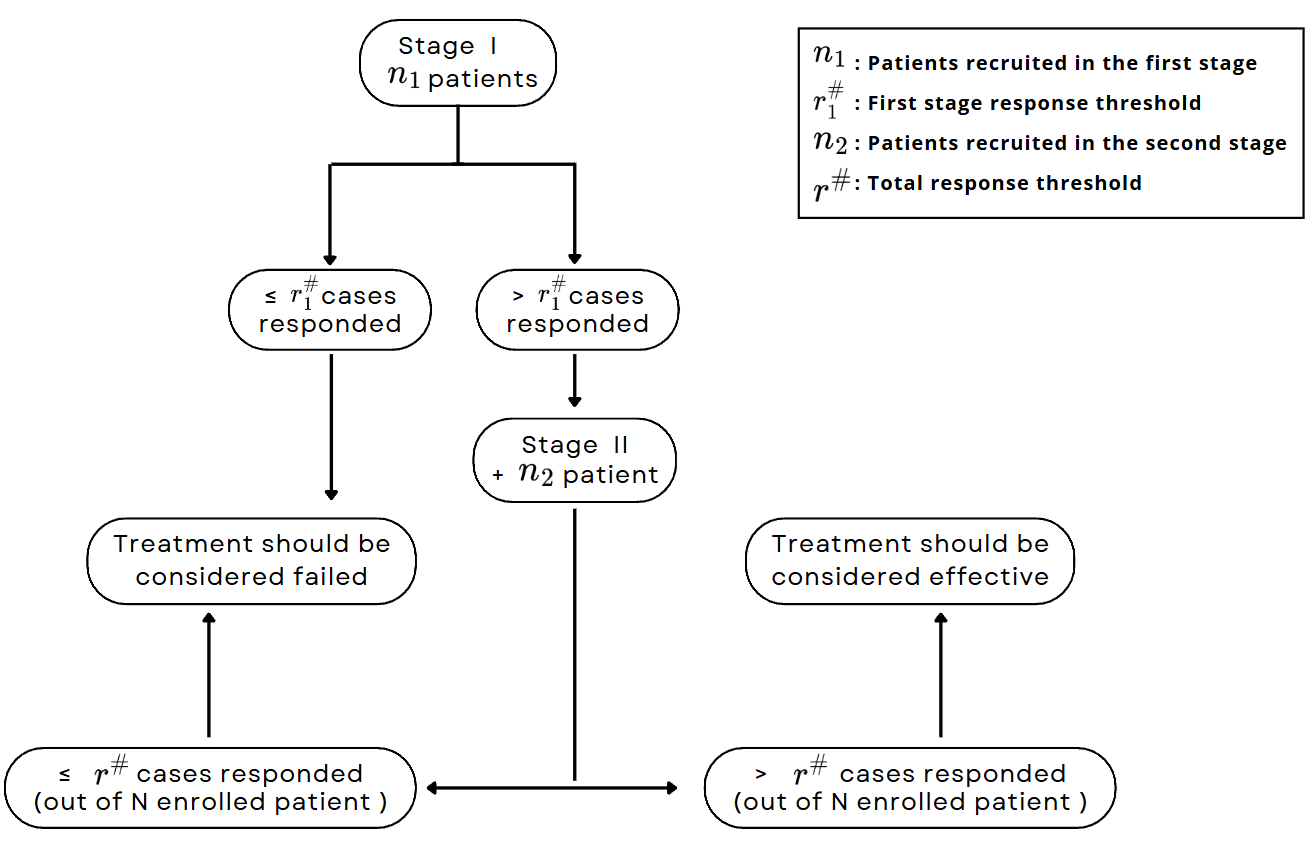
\includegraphics[width=1\linewidth, trim=0cm 0cm 0cm 0cm, clip]{simon optimal plot.png} % 调整 trim 参数裁剪图片边缘
    %\caption{PSO 演算法示意圖}
    \label{fig:pso}
\end{figure}
\end{frame}




\begin{frame}{Literature Review: Simon's Two-Stage Design}
\begin{columns}
    % Left content
    \column{0.6\textwidth}
    \begin{block}{Phase II Trials Based on Hypothesis Testing}
        \begin{itemize}
            \item \( H_0 : p \leq p_0 \)
            \item \( H_1 : p \geq p_1 \)
        \end{itemize}
        \vspace{0.3cm}
        \begin{itemize}
            \item \( p_0 \): Disinterested response level
            \item \( p_1 \): Desired response level
        \end{itemize}
    \end{block}

    % Right content
    \column{0.4\textwidth}
    \begin{block}{Considerations}
        \begin{itemize}
            \item Constrained by \( \alpha \) and \( \beta \)
            \item Minimizing the number of patients receiving low-efficacy treatment
        \end{itemize}
    \end{block}
\end{columns}

\vspace{0.5cm}
\end{frame}



\section{Expected Sample Size}
\begin{frame}{Probability of Early Termination at Each Stage}
\begin{itemize}
    \item Assume each patient's response is a binary random variable with a success probability of \( p \).
    \item Let \( b(x; n, p) \) denote the probability of having \( x \) responses among \( n \) patients. The binomial distribution formula is:
    \[
    b(x; n, p) = \binom{n}{x} p^x (1 - p)^{n - x}
    \]
\end{itemize}
\end{frame}


\begin{frame}{Probability of Early Termination (PET) in \( K \)-Stage Design}
\begin{itemize}
        \item The formula is as follows:
        \[
        \hspace{-1.5cm}
        PET_k(p) = 
		\underbrace{
    	\sum_{x_1 = L_1}^{U_1} \sum_{x_2 = L_2}^{U_2} \cdots \sum_{x_{k-1} = L_{k-1}}^{U_{k-1}}
		}_{k-1 \text{ Summations}}
		\left[ \prod_{s=1}^{k-1} b(x_s; n_s, p) \right]
		B\left( r_k = \sum_{s=1}^{k-1} x_s, n_k, p \right)
		\]
        \item \scriptsize
        where:
	\begin{itemize}
            \item \( b(x_s; n_s, p) \) represents the binomial probability at stage \( s \).
            \item \( L_j \) and \( U_j \) are the lower and upper bounds of stage \( j \), respectively.
            \item \( B(\cdot) \) is the cumulative distribution function of the binomial distribution.
    \end{itemize}
\end{itemize}
\end{frame}


\begin{frame}{Probability of Treatment Rejection and Expected Sample Size}
\begin{itemize}
    \item \textbf{Probability of Treatment Rejection at the End of the Third Stage}:
    \[
    \sum_{x_1 = r_1 + 1}^{\min[n_1, r_3]} \sum_{x_2 = r_2 + 1 - x_1}^{\min[n_2, r_3 - x_1]} b(x_1; n_1, p) b(x_2; n_2, p) B(r_3 - x_1 - x_2; n_3, p)
    \]
    \item \textbf{Expected Sample Size (EN)}:
    \[
    EN = n_1 + (1 - PET_1) n_2 + (1 - PET_{\text{2}}) n_3
    \]
\end{itemize}
\end{frame}


\begin{frame}{Total Combination Possibilities}
\begin{itemize}
    \item 2-Stage Design: \hspace*{1.5cm}\( 1,105,524 \) possibilities
    \item 3-Stage Design: \hspace*{1.12cm}\( 213,672,935 \) possibilities
    \item 4-Stage Design: \hspace*{0.56cm}\( 22,546,940,047 \) possibilities
    \item 5-Stage Design: \( 1,530,973,869,444 \) possibilities

    As the number of stages increases, the number of combinations becomes larger, making clinical design more complex.
\end{itemize}

\footnotesize % 缩小字体
\textbf{Note:} Enumeration range: \\
\hspace*{1cm} Total sample size \( N = n_1 + \ldots + n_k \), where \( 30 \leq N \leq 70 \). % 添加备注
\end{frame}


\section{PSO Algorithm}
\begin{frame}
\frametitle{PSO(Particle Swarm Optimization)}
\begin{figure}
    \centering
    \hspace{0 cm} % 调整水平偏移
    \vspace{2 cm} % 调整垂直偏移
    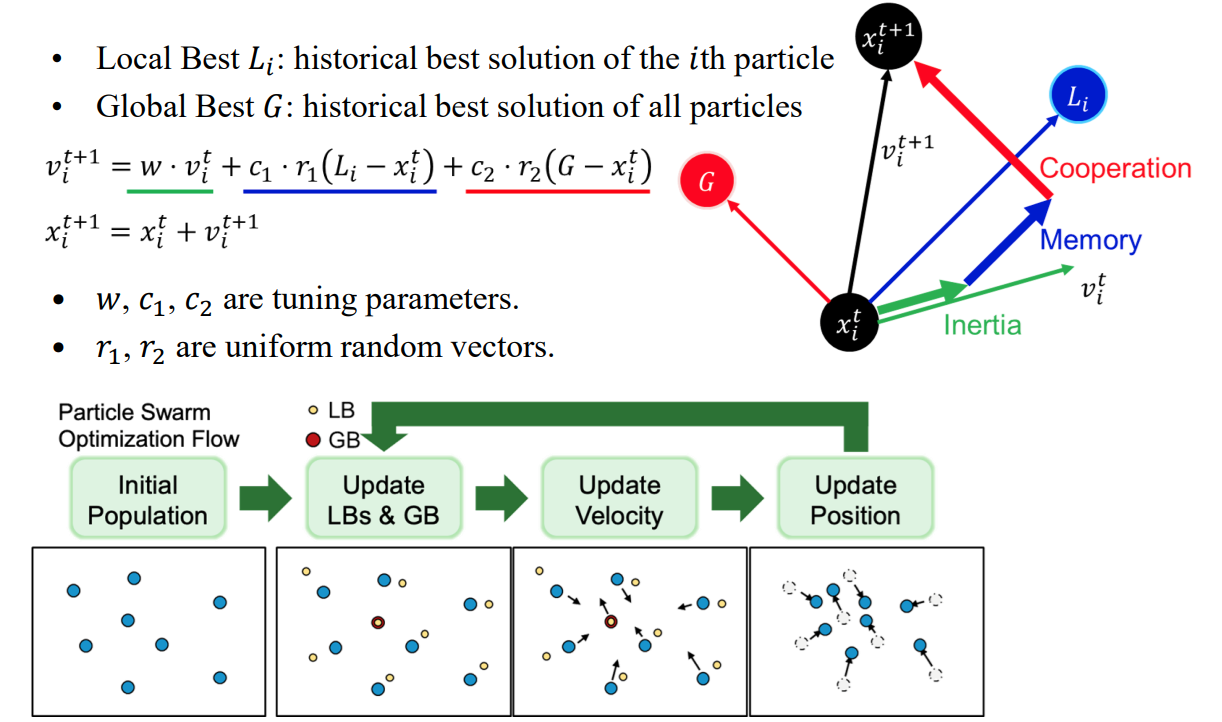
\includegraphics[width=1.05\linewidth]{PSO.png} % 確保圖片在與.tex文件相同的目錄
    %\caption{PSO 演算法示意圖}
    \label{fig:pso}
\end{figure}
\end{frame}



\section{Existing results}
\begin{frame}
\frametitle{Four-stage Optimal Design}
% 四階段表格
\begin{center}
\resizebox{1\linewidth}{!}{% 将 0.9 调整为 0.95 或 0.85 以控制缩放比例
\begin{tabular}{|c|c|c|c|c|c|>{\columncolor{yellow}}c|c|c|c|}
\hline
$p_0$ & $p_1$ & Stage 1 & Stage 2 & Stage 3 & Stage 4 & EN($p_0$) & $PET_1$($p_0$) & $PET_2$($p_0$) & $PET_3$($p_0$) \\
\hline
0.05 & 0.25 & 0/9 & 0/17 & 1/18 & 2/26 & 13.78 & 0.63 & 0.63 & 0.82 \\
0.1 & 0.3 & 0/11 & 1/15 & 2/19 & 4/26 & 17.37 & 0.31 & 0.57 & 0.73 \\
0.15 & 0.35 & 0/9 & 2/16 & 4/26 & 7/33 & 20.55 & 0.23 & 0.58 & 0.72 \\
0.2 & 0.4 & 1/10 & 4/21 & 7/30 & 11/43 & 22.73 & 0.38 & 0.63 & 0.8 \\
0.25 & 0.45 & 1/10 & 4/18 & 8/28 & 14/45 & 24.42 & 0.24 & 0.54 & 0.78 \\
0.3 & 0.5 & 2/11 & 6/21 & 11/33 & 17/46 & 25.77 & 0.31 & 0.59 & 0.78 \\
0.35 & 0.55 & 4/14 & 10/27 & 15/38 & 20/48 & 26.55 & 0.42 & 0.7 & 0.82 \\
0.4 & 0.6 & 4/13 & 10/24 & 16/36 & 23/49 & 26.29 & 0.3 & 0.62 & 0.75 \\
0.45 & 0.65 & 3/10 & 9/20 & 16/33 & 25/48 & 25.81 & 0.27 & 0.61 & 0.77 \\
0.5 & 0.7 & 4/11 & 8/17 & 15/28 & 26/45 & 24.96 & 0.27 & 0.52 & 0.75 \\
0.55 & 0.75 & 5/11 & 10/18 & 19/32 & 28/45 & 23.2 & 0.37 & 0.63 & 0.76 \\
0.6 & 0.8 & 5/10 & 9/15 & 17/27 & 27/40 & 20.91 & 0.37 & 0.61 & 0.76 \\
0.65 & 0.85 & 5/9 & 13/19 & 20/28 & 24/33 & 18.32 & 0.39 & 0.72 & 0.75 \\
0.7 & 0.9 & 1/3 & 6/9 & 15/20 & 24/31 & 14.72 & 0.22 & 0.56 & 0.8 \\
0.75 & 0.95 & 3/5 & 6/8 & 11/14 & 16/19 & 10.23 & 0.37 & 0.63 & 0.77 \\
\hline
\multicolumn{10}{|l|}{$p_1 -  p_0 =0.20$ and $\alpha = 0.1$ , $\beta = 0.1$} \\ % 这里指定10列，并放在一个完整的表格行中
\hline
\end{tabular}
}
\end{center}
\end{frame}

\begin{frame}
\frametitle{Four-stage Minimax Design}
% Minimax Design 表格
\begin{center}
\resizebox{1\linewidth}{!}{% 将 0.9 调整为 0.95 或 0.85 以控制缩放比例
\begin{tabular}{|c|c|c|c|c|c|>{\columncolor{yellow}}c|c|c|c|}
\hline
$P_0$ & $P_1$ & Stage 1 & Stage 2 & Stage 3 & Stage 4 & EN($p_0$) & $PET_1$($p_0$) & $PET_2$($p_0$) & $PET_3$($p_0$) \\
\hline
0.05 & 0.25 & 0/13 & 0/15 & 1/18 & 2/20 & 15.86 & 0.51 & 0.51 & 0.79 \\
0.1 & 0.3 & 0/12 & 1/16 & 3/24 & 4/25 & 18.83 & 0.28 & 0.53 & 0.8 \\ 
0.15 & 0.35 & 0/11 & 2/17 & 4/25 & 7/32 & 21.75 & 0.17 & 0.53 & 0.72 \\
0.2 & 0.4 & 1/13 & 3/20 & 6/29 & 10/36 & 25.7 & 0.23 & 0.44 & 0.67 \\
0.25 & 0.45 & 8/29 & 9/31 & 11/35 & 12/37 & 30.71 & 0.71 & 0.78 & 0.87 \\
0.3 & 0.5 & 3/20 & 8/30 & 12/36 & 15/39 & 33.1 & 0.11 & 0.44 & 0.74 \\
0.35 & 0.55 & 3/14 & 6/20 & 10/27 & 18/42 & 27.36 & 0.22 & 0.43 & 0.68 \\
0.4 & 0.6 & 6/20 & 9/25 & 12/30 & 20/41 & 30.82 & 0.31 & 0.52 & 0.73 \\
0.45 & 0.65 & 5/15 & 8/20 & 14/30 & 22/41 & 27.97 & 0.26 & 0.43 & 0.67 \\
0.5 & 0.7 & 5/14 & 10/22 & 17/32 & 23/39 & 27.93 & 0.21 & 0.44 & 0.72 \\
0.55 & 0.75 & 6/13 & 13/24 & 22/35 & 24/38 & 25 & 0.36 & 0.59 & 0.87 \\
0.6 & 0.8 & 4/9 & 12/20 & 16/25 & 24/35 & 21.54 & 0.27 & 0.61 & 0.75 \\ 
0.65 & 0.85 & 7/12 & 11/17 & 15/22 & 23/31 & 19.32 & 0.42 & 0.6 & 0.73 \\
0.7 & 0.9 & 5/9 & 11/16 & 15/20 & 20/25 & 17.02 & 0.27 & 0.56 & 0.77 \\
0.75 & 0.95 & 3/5 & 6/8 & 11/14 & 16/19 & 10.23 & 0.37 & 0.63 & 0.77 \\
\hline
\multicolumn{10}{|l|}{$p_1 -  p_0 =0.20$ and $\alpha = 0.1$ , $\beta = 0.1$} \\ % 这里指定10列，并放在一个完整的表格行中
\hline
\end{tabular}
}
\end{center}
\end{frame}


\begin{frame}
\frametitle{EN($p_0$) Comparison between 3 \& 4-stage Designs}
\vspace{-0.5cm} % 调整此值以控制上移的距离
\begin{center}
\resizebox{\linewidth}{!}{%
\begin{tabular}{|c|c|c|c|c|c|c|c|}
\hline
\multirow{2}{*}{$P_0$} & \multirow{2}{*}{$P_1$} & \multicolumn{2}{c|}{\cellcolor{cyan}EN($p_0$) (Optimal)} & \multirow{2}{*}{Variation} & \multicolumn{2}{c|}{\cellcolor{yellow}EN($p_0$) (Minimax)} & \multirow{2}{*}{Variation} \\
\cline{3-4}\cline{6-7}
& & 3-stage & 4-stage & & 3-stage & 4-stage & \\
\hline
0.05 & 0.25 & 13.78 & 13.78 & 0 & 15.86 & 15.86 & 0 \\
0.1 & 0.3 & 17.79 & 17.37 & -0.42 & 19.1 & 18.83 & -0.27 \\ % 更新后的4-stage数据
0.15 & 0.35 & 21.11 & 20.55 & -0.56 & 22.23 & 21.75 & -0.48 \\
0.2 & 0.4 & 23.86 & 22.73 & -1.13 & 26.41 & 25.7 & -0.71 \\
0.25 & 0.45 & 25.55 & 24.42 & -1.13 & 29.83 & 29.1 & -0.73 \\
0.3 & 0.5 & 26.75 & 25.77 & -0.98 & 33.71 & 33.1 & -0.61 \\
0.35 & 0.55 & 27.84 & 26.55 & -1.29 & 28.59 & 27.36 & -1.23 \\
0.4 & 0.6 & 29.81 & 26.29 & -3.52 & 32.48 & 30.82 & -1.66 \\
0.45 & 0.65 & 27.22 & 25.81 & -1.41 & 28.94 & 27.97 & -0.97 \\
0.5 & 0.7 & 26.37 & 24.96 & -1.41 & 29 & 27.93 & -1.07 \\
0.55 & 0.75 & 24.36 & 23.2 & -1.16 & 27.74 & 25 & -2.74 \\
0.6 & 0.8 & 22.3 & 20.91 & -1.39 & 22.97 & 21.54 & -1.43 \\ % 更新后的4-stage数据
0.65 & 0.85 & 19.23 & 18.32 & -0.91 & 22.22 & 19.32 & -2.9 \\
0.7 & 0.9 & 15.45 & 14.72 & -0.73 & 17.85 & 17.02 & -0.83 \\
0.75 & 0.95 & 10.94 & 10.23 & -0.71 & 10.94 & 10.23 & 0 \\
\hline
\end{tabular}
}
\end{center}
\end{frame}

\begin{frame}
\frametitle{EN($p_0$) vs Cumulative CPU Time for Different PSO}
\begin{figure}
    \centering
    \hspace*{-0.8cm} % 向左移動 1 cm，調整此值來改變偏移程度
    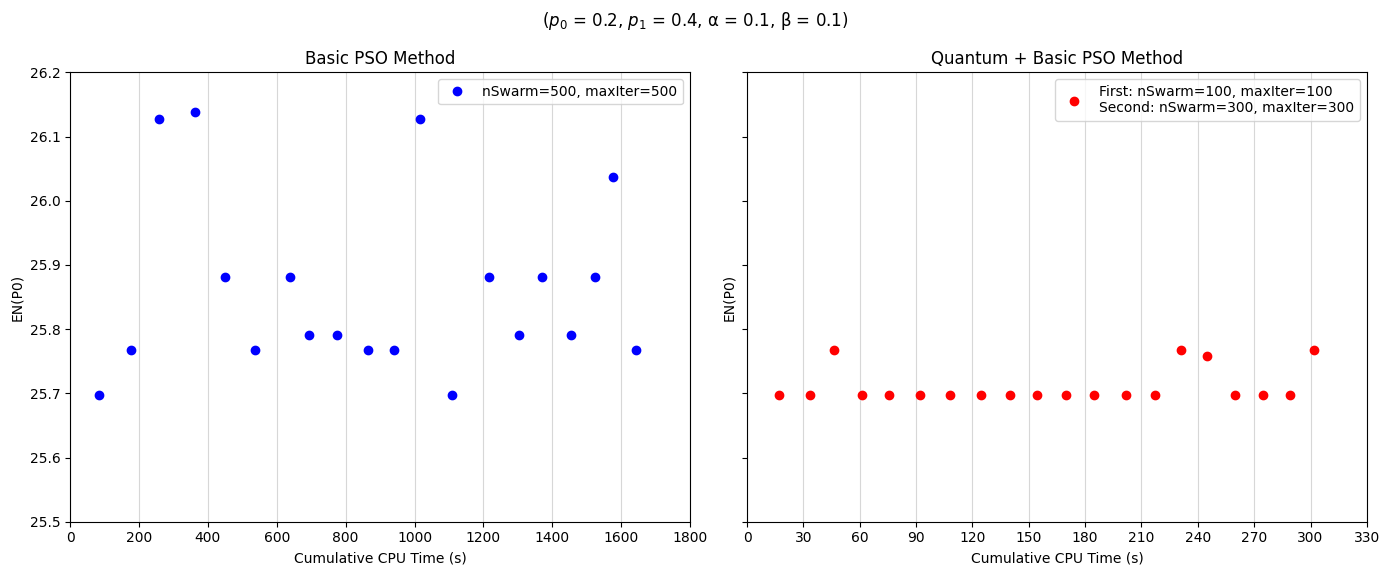
\includegraphics[width=1.15\linewidth]{Different PSO Methods.png} % 確保圖片在與.tex文件相同的目錄
\end{figure}
\end{frame}


\section{Discussions, Challenges, and Future Plans}
\begin{frame}
\frametitle{Discussions, Challenges, and Future Plans}
\begin{itemize}
    \item \textbf{Challenges in Algorithm Implementation}:
    \begin{itemize}
        \item Stability issues, convergence speed, and sensitivity to parameters .
        \item Inconsistent results across multiple runs.
    \end{itemize}
    
    \item \textbf{Future Research Directions}:
    \begin{itemize}
        \item Enhancing algorithm stability and convergence efficiency.
        \item Investigating other relevant clinical trial designs or incorporating additional literature for further improvements.
    \end{itemize}
\end{itemize}
\end{frame}


\begin{frame}{References}
\small % 或者使用 \footnotesize 进一步缩小字体
\begin{itemize}
	\item Atkinson, A., Donev, A., Tobias, R. (2007). Optimum experimental designs, with SAS. OUP Oxford. (pp. 58-69, Chapter 6; pp. 119-147, Chapters 9-10).
	\item Chen, T. T. (1997). Optimal three-stage designs for phase II cancer clinical trials. Statistics in medicine, 16(23):2701–2711.
	\item Qiu, J., Chen, R.-B., Wang, W., and Wong, W. K. (2014). Using animal instincts to design efficient biomedical studies via particle swarm optimization. Swarm and evolutionary computation, 18:1–10.
    \item Simon, R. (1989). Optimal two-stage designs for phase ii clinical trials. Controlled clinical trials, 10(1):1–10.
    \item Yang, X.-S. (2010). Engineering optimization: an introduction with metaheuristic applications, pp. 29-35.
    
\end{itemize}
\end{frame}


\end{document}


